\documentclass[11pt,letterpaper]{article}

\usepackage[letterpaper,margin=0.8in,nohead]{geometry}

\usepackage[colorlinks]{hyperref}
\usepackage{url}
\usepackage{breakurl}

\hypersetup{
    colorlinks,
    linkcolor={red},
    citecolor={red},
    urlcolor={blue}
}

\usepackage{verbatim}
\usepackage{fancyvrb}
\usepackage{scrextend}
\usepackage{enumitem}
\usepackage{url}
\usepackage{subcaption}

\usepackage{filecontents}
%\usepackage{natbib}
%\nobibliography*

\usepackage{caption}
\usepackage{graphicx}

\usepackage{changepage}   % for the adjustwidth environment

\newenvironment{answer}{\em \color{blue} \begin{adjustwidth}{1cm}{1cm}}{\end{adjustwidth}}

% math
\usepackage{amsthm,amsmath}
\usepackage{amsfonts}

\newcommand{\mc}[1]{\mathcal{#1}}	% Mechanisms / Algorithms
\newcommand{\rv}[1]{\mathbf{#1}}    % Random variable

\newcommand{\pr}[1]{\mathrm{Pr}\{#1\}} % Probability

\newtheorem{corollary}{\bf Corollary}%[theorem]
\newtheorem{lemma}{\bf Lemma}%[theorem]
\newtheorem{definition}{\bf Definition}%[section]

\newtheorem{observation}{\bf Observation}%[theorem]



% load cleveref last!
\usepackage[capitalise]{cleveref}

\crefname{observation}{Observation}{Observations}


\begin{document}

\title{EN4720: Security in Cyber-Physical Systems \\ Programming Assignment}

%% This is an individual assignment!!
%% TODO: put your name and index number here here!
\author{ \textcolor{blue}{Name: Akila Rajapaksha} \\ \textcolor{blue}{Index No: 190484T}}

\maketitle

\begin{center}
	\color{red}\bf This is an individual assignment! \\ Due Date: 7 April 2024 by 11.59 PM
\end{center}

\section*{Instructions}
%

Please read the instructions and questions carefully. Read the whole document before attempting to answer to make sure you don't miss any important instructions. 

\subsection*{Submission}
Write your answers directly in the space provided. Compile the tex document and submit the resulting PDF together with the source codes and all the generated files in the process in a single zip file through Moodle.

\medskip
\noindent Be sure to include the short demo video as well (Problem 4) in the zip file.


\newpage
\section*{Problem 1: Implementing Symmetric-Key Encryption ({25 pts})}
%

\subsubsection*{Instructions}
%

\noindent In this assignment, you will write a few lines of Python code. You are encouraged to use Python3. You will need the PyCryptodome library to run the provided code. Please refer to resources specific to your operating system and environment for installation instructions\footnote{\url{https://pypi.org/project/pycryptodome/} See also:  \url{https://www.pycryptodome.org/en/latest/index.html}.}. For example, you can use: \texttt{pip3 install pycryptodome} to install PyCryptodome with Python3 under Linux or in your PowerShell instance. 

\subsection*{Assignment Files}
The assignment archive contains the following Python source files:

\begin{itemize}[nolistsep]
	\item \texttt{encrypt\_phrase.py} This file contains the skeleton code required for Task 1.
	\item \texttt{aes\_encryption.py} This file contains the skeleton code required for Task 2.\\
\end{itemize}

\subsection*{Task 1: Implementing basic encryption using AES with Python scripting}

In this task, you will be given a partially developed Python script ``\texttt{encrypt\_phrase.py}''. Follow the given guidelines and complete the script to encrypt a phrase given by the user.

\medskip
\noindent You can make use of the AES function under Crypto.Cipher package. However, you're not allowed to make use of the Fernet function.

\medskip
\noindent The script should follow the guidance notes mentioned below, provided to guide and assist you to complete the task. 

\begin{enumerate}
    \item Create a Key.
    \item Create the Cipher object using the Key (AES mode is CBC).
    \item Request the user to enter a message that they want to be encrypted.
    \item Encrypt the message using the generated cipher.
    \item Provide the ciphertext along with the key as the output.
\end{enumerate}

\noindent \textbf{Questions}
\medskip
\begin{enumerate}
    \item What would be the ideal byte length to be used in the random number generator? Define the logic behind the selection of the value. 
    \begin{answer}
		%% TODO: Write your answer here.	
		Your answer here.
	\end{answer}
    \item Define the technique used to overcome the challenge with the size of data blocks that occur when dealing with block ciphers. 
    \begin{answer}
		%% TODO: Write your answer here.	
		Your answer here.
	\end{answer}
    \item Complete the Python script and provide the following information with evidence. (Code/output snip of the PowerShell/Bash terminal     instance)\\ 
        Phrase: \\
        Key: \\
        Cipher-text:
        \begin{answer}
		%% TODO: Write your answer here.	
		Your answer here.
	\end{answer}
    \item Modify the provided Python script to incorporate the use of a unique Initialization Vector (IV) for each encryption operation in AES-CBC mode. Explain how this modification enhances the security of the encryption process.
    \begin{answer}
		%% TODO: Write your answer here.	
		Your answer here.
	\end{answer}

\end{enumerate}

\subsection*{Task 2: Implementing encryption using AES256}
%

In this task, you will be assigned a partially developed Python script ``\texttt{aes\_encryption.py}''. Follow the given guidelines and complete the script to encrypt a phrase given by the user.

\medskip
\noindent You are tasked with developing a Python script (with the use of the skeleton code provided), which encrypts a plaintext phrase and generate the ciphertext using a key. You can make use of the Fernet function in the Cryptography module. This task will rely upon the use of concepts and techniques utilized in Task 1.  

\medskip
The script should follow the guidance notes mentioned below, provided to guide and assist you in achieving the task.

\begin{enumerate}
    \item Generate the Key using Fernet.
    \item Complete the encryption function.
    \item Request the user to enter the phrase that they want to be encrypted
    \item Provide the ciphertext along with the key as the output.
\end{enumerate}

\noindent \textbf{Questions}
\medskip
\begin{enumerate}
    \item What are the characteristics of a key generated by the Fernet function compared to the key generated in Task 1?
    \begin{answer}
		%% TODO: Write your answer here.	
		Your answer here.
	\end{answer}
    \item Why Fernet is not suitable to be used for the encryption of larger-sized files?
    \begin{answer}
		%% TODO: Write your answer here.	
		Your answer here.
	\end{answer}
    \item What technique is utilized by Fernet to introduce randomness to the encryption process?
    \begin{answer}
		%% TODO: Write your answer here.	
		Your answer here.
	\end{answer}
    \item How can Randomization and Padding minimize the impact of AES-256-CBC against side-channel attacks?
    \begin{answer}
		%% TODO: Write your answer here.	
		Your answer here.
	\end{answer}

\end{enumerate}


\newpage
\section*{Problem 2: Keys and Certificates with OpenSSL ({20 pts})}

In this problem, you will complete a set of tasks designed around the use of OpenSSL to give an insight into the use of encryption in applications. The tasks will form a guided lab scenario with commands to be completed fully for execution, in accordance with instructions. Proceed to answer the questions based on the findings and outcomes of the executed tasks and generated certificates.

\medskip
\noindent This problem will make use of the following technology components. 
\smallskip
\begin{itemize}[nolistsep]
	\item Oracle VirtualBox.
	\item Ubuntu LTS Server. 
	\item OpenSSL package.
\end{itemize} 

\smallskip
\noindent Please refer to resources specific to your operating system and environment for installation instructions for VirtualBox\footnote{\url{https://www.virtualbox.org/manual/ch02.html} } and setting up Ubuntu LTS as a VM\footnote{\url{https://ubuntu.com/tutorials/how-to-run-ubuntu-desktop-on-a-virtual-machine-using-virtualbox}}.\

%%%%%%%%%%%%%%%%%%%%%%%%%%%%%%%%%%%%%%%%%%% 2.1 %%%%%%%%%%%%%%%%%%%%%%%%%%%%%%%%%%%%%%%%%%%%%%%%%%%%%%%%%%%%%%%%
\subsection*{Task 1 : Generating Private/Public Key pair with OpenSSL}

This task will revolve around the use of OpenSSL to generate a public and private key pair using a custom set of parameters. Further, the commands given are incomplete and you are required to go through the documentation and use necessary changes and additions to the command set. 

The problem will generate a Private key followed by a Public key. Add all necessary screenshots of each step. 
%

\begin{enumerate}

    \item Create a Protected Private Key based on the following parameters. \\(Key Length: 4096, Encryption: AES192, Algorithm: RSA) 
    \begin{Verbatim}
    $ openssl genpkey  -algorithm RSA -pkeyopt -out <student_no>-private-key.pem
    \end{Verbatim}

    \begin{figure}[h]
        \centering
        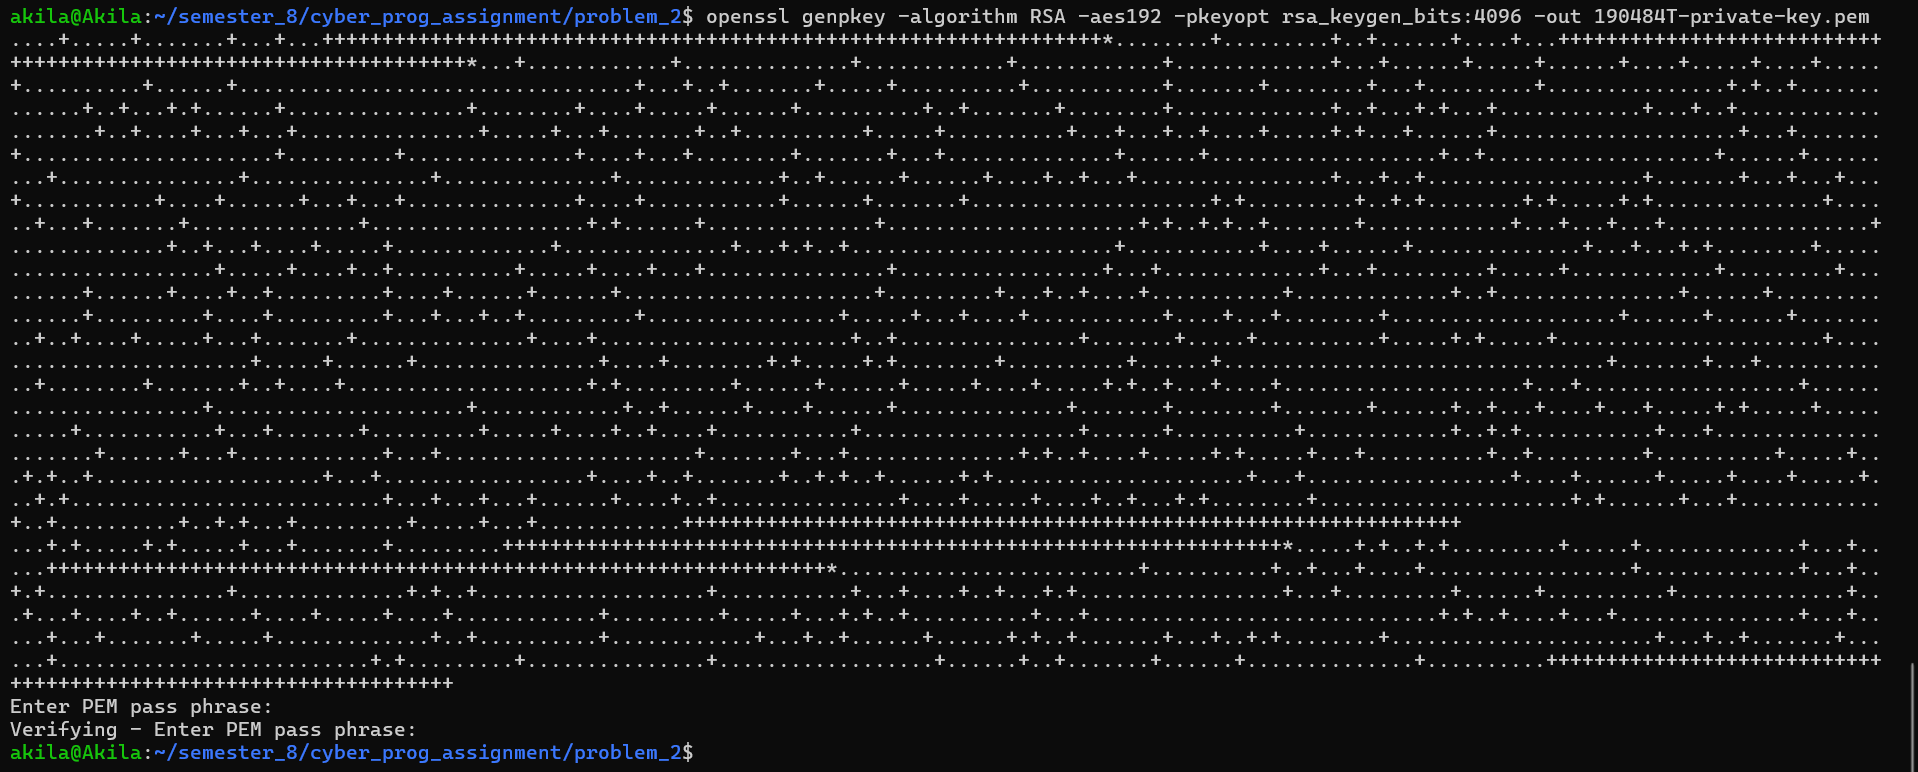
\includegraphics[width=\textwidth]{images/question_2-image_1.png}
        \caption{creating a private key}
        \label{fig:enter-label}
    \end{figure}
        
    \item Create a Public key using the Private key generated in the previous task. 
    \begin{Verbatim}
    $ openssl pkey -in  -out <student_no>-public-key.pem -pubout
    \end{Verbatim}

    \item Describe each segment in the commands that you have executed for previous questions. 
    \begin{answer}
	
		%% TODO: Write your answer here.	
		Your answer here.
		
	\end{answer}
     \item Explain the components found in the \textless student\_no\textgreater-private-key.pem. 
     \begin{answer}
	
		%% TODO: Write your answer here.	
		Your answer here.
		
	\end{answer}
    \item Elaborate on the reason for the existence of all the parameters in addition to the modulus, public exponent and private exponent in the private key, with respect to the key length utilized in the above key generation scenario.
    \begin{answer}
	
		%% TODO: Write your answer here.	
		Your answer here.
		
	\end{answer}
    \item What are the security considerations that need to be adopted when storing and handling private keys in this format?
    \begin{answer}
	
		%% TODO: Write your answer here.	
		Your answer here.
		
	\end{answer}

\end{enumerate}

\newpage
%%%%%%%%%%%%%%%%%%%%%%%%%%%%%%%%%%%%%%%%%%% 2.2 %%%%%%%%%%%%%%%%%%%%%%%%%%%%%%%%%%%%%%%%%%%%%%%%%%%%%%%%%%%%%%%%
\subsection*{Task 2 : Generate a Self-signed SSL Certificate with OpenSSL}
%
This problem will revolve around the use of OpenSSL to generate an SSL certificate with self-signing. The commands given are incomplete and you are required to go through the documentation and use necessary changes and additions to the command set.

The tasks will generate a key, certificate signing request (CSR) followed by the self-signed SSL certificate. Add all necessary screenshots of each step. 

\begin{enumerate}

   \item Create the Key based on the following parameters to be used for the CSR. \\(Key Length: 4096, Encryption: DES3)
    \begin{Verbatim}
    $ openssl genrsa -out <student_no>-CSR_Key.key 
    \end{Verbatim}
        
    \item Create the CSR using the key generated in the previous task. 
    \\ (Org - Skills Surf, OU - Cryptography, CN - \textless student\_no\textgreater)
    \begin{Verbatim}
    $ openssl req -new -key <student_no>-CSR_Key.key -out <student_no>-CSR.csr
    \end{Verbatim}

    \item Create the self-signed SSL certificate using the CSR generated in the previous task. 
    \\ (Validity - 180 days)
    \begin{Verbatim}
    $ openssl x509 -req -in -signkey -out <student_no>-Certificate.crt
    \end{Verbatim}

    \item Elaborate on the critical role of Cipher Suites in SSL certificate with respect to the impact on digital communication performance and overall security. 
    \begin{answer}
	
		%% TODO: Write your answer here.	
		Your answer here.
		
	\end{answer}
    \item How is the certificate chain constructed, and what is the role of the root certificate, intermediate certificates, and the end-entity certificate?
    \begin{answer}
	
		%% TODO: Write your answer here.	
		Your answer here.
		
	\end{answer}
    \item What mechanisms are in place for certificate revocation, in an event where either the private key has been compromised or the certificate has an invalidation?
    \begin{answer}
	
		%% TODO: Write your answer here.	
		Your answer here.
		
	\end{answer}
    \item What is the role of Hardware Security Module (HSM)?
    \begin{answer}
	
		%% TODO: Write your answer here.	
		Your answer here.
		
	\end{answer}

\end{enumerate}

%%%%%%%%%%%%%%%%%%%%%%%%%%%%%%%%%%%%%%%%%%%%%%%%%%% Problem 4 %%%%%%%%%%%%%%%%%%%%%%%%%%%%%%%%%%%%%%%%%%%%%%%%%%%
\newpage
\section*{Problem 3:  Encryption with Certificates ({20 pts})}

\subsubsection*{Instructions}

In this problem, you will write a few lines of Python code. You are encouraged to use Python3. You will need the PyCryptodome library to run the provided code. Please refer to resources specific to your operating system and environment for installation instructions\footnote{\url{https://pypi.org/project/pycryptodome/} See also:  \url{https://www.pycryptodome.org/en/latest/index.html}.}. For example, you can use: \texttt{pip3 install pycryptodome} to install PyCryptodome with Python3 under Linux or in your PowerShell instance. 

\medskip
\noindent You can use PKCS1\_OAEP from Crypto.Cipher and RAS from Crypto.PublicKey for this task. 

\medskip
\subsubsection*{Assignment Files}
The assignment archive contains the following source files:

\begin{itemize}[nolistsep]
	\item \texttt{encrypt\_file.py} This file contains the skeleton code required for Task 1.
	\item \texttt{decrypt\_file.py} This file contains the skeleton code required for Task 2.
        \item \texttt{input.txt} Update this with your information.
        \item \texttt{cipher.txt} This file should contain the encrypted input text.
        \item \texttt{output.txt} This file should contain the decrypted text.
\end{itemize}


\subsubsection*{Prerequisites}

\noindent Availability of pre-generated Private and Public Key pair. Make use of the instructions and knowledge gained in Assessment 2 Task 1. Do not encrypt the private key for this task. 

%%%%%%%%%%%%%%%%%%%%%%%%%%%%%%%%%%%%%%%%%%% 3.1 %%%%%%%%%%%%%%%%%%%%%%%%%%%%%%%%%%%%%%%%%%%%%%%%%%%%%%%%%%%%%%%%
\subsection*{Task 1 : Encryption of Files using a Public Key.}

In this task, you will be assigned a partially developed Python script ``\texttt{encrypt\_file.py}''. You are to follow the given guidelines and complete the script to get the desired outcome of encryption of a file given by the user.

\medskip
\noindent You are tasked with developing a Python script (with the use of the skeleton code provided), that makes use of the following specific packages and commands to encrypt a file using a private key in the format of .pem file.

\medskip
\noindent The script should follow the guidance notes mentioned below, provided to guide and assist you to complete the task itself. 

\begin{enumerate}
    \item Request the user to enter the file to be encrypted, public key and output path. 
    \item Read the content of the file to be encrypted and store in a variable.
    \item Import the Public Key, used for the encryption function.
    \item Encrypt the file (stored in a variable).
    \item Write the encrypted file in the designed location as defined by the user.
    \item Now create another input file called \texttt{sample\_long.txt} and enter a random paragraph which has more than 1000 characters.
    \item Do the encryption for that file as well.
\end{enumerate}

\newpage

\noindent \textbf{Questions}
\medskip
\begin{enumerate}
    \item What is the output you get from the last step?
        \begin{answer}
	
		%% TODO: Write your answer here.	
		Your answer here.
		
	\end{answer}
    \item What is the maximum plain-text length(in Bytes) supported by this encryption under the parameters used in this problem?
        \begin{answer}
	
		%% TODO: Write your answer here.	
		Your answer here.
		
	\end{answer}
    \item State the equation which gives the maximum plain-text length. Derivations are not needed.
        \begin{answer}
	
		%% TODO: Write your answer here.	
		Your answer here.
		
	\end{answer}
    \item Compare and contrast between the JSON Web Key and PEM key formats.
        \begin{answer}
	
		%% TODO: Write your answer here.	
		Your answer here.
		
	\end{answer}
    \item How to protect PEM keys from factoring attacks?
        \begin{answer}
	
		%% TODO: Write your answer here.	
		Your answer here.
		
	\end{answer}

\end{enumerate}

%%%%%%%%%%%%%%%%%%%%%%%%%%%%%%%%%%%%%%%%%%% 3.2 %%%%%%%%%%%%%%%%%%%%%%%%%%%%%%%%%%%%%%%%%%%%%%%%%%%%%%%%%%%%%%%%

\subsection*{Task 2: Decryption of Files using a Private Key.}
%
In this task, you will be assigned a partially developed Python script ``\texttt{decrypt\_file.py}''. You are to follow the given guidelines and complete the script to get the desired outcome of the decryption of an encrypted file given by the user.

\medskip
You are tasked with developing a Python script (with the use of the skeleton code provided), which makes use of the following specific packages and commands to decrypt a file that was encrypted in the previous task using the associated private key in the format of .pem file.  

\medskip
The script should follow the guidance notes mentioned below, provided to guide and assist you in achieving the task.

\begin{enumerate}
    \item Request the user to enter the file to be decrypted, private key and output path. 
    \item Read the content of the file to be decrypted and store in a variable. 
    \item Import the Private Key, used for the decryption function. 
    \item Decrypt the file (stored in variable) 
    \item Write the decrypted file in the designed location as defined by the user.

\end{enumerate}

\noindent \textbf{Questions}
\medskip
\begin{enumerate}
    \item Upload screen shots of the \texttt{input.txt}, \texttt{cipher.txt} and \texttt{output.txt} files.
        \begin{answer}
	
		%% TODO: Write your answer here.	
		Your answer here.
		
	\end{answer}
    \item What techniques are available to ensure the authenticity of an encrypted message in asymmetric encryption?
        \begin{answer}
	
		%% TODO: Write your answer here.	
		Your answer here.
		
	\end{answer}
    \item Elaborate on the relationship between PKI and Digital Signatures in the context of Certificates. 
        \begin{answer}
	
		%% TODO: Write your answer here.	
		Your answer here.
		
	\end{answer}
\end{enumerate}

%%%%%%%%%%%%%%%%%%%%%%%%%%%%%%%%%%%%%%%%%%% END 3  %%%%%%%%%%%%%%%%%%%%%%%%%%%%%%%%%%%%%%%%%%%%%%%%%%%%%%%%%%%%%%

\newpage

%%%%%%%%%%%%%%%%%%%%%%%%%%%%%%%%%%%%%%%%%%%%%%%%%%% Problem 4 %%%%%%%%%%%%%%%%%%%%%%%%%%%%%%%%%%%%%%%%%%%%%%%%%%%
\section*{Problem 4: Hybrid Encryption ({35 pts})}
In the Task 1 of the last problem, you observed that plain-text length is a limitation  in the RSA algorithm. Therefore in this problem you will learn how such limitations are addressed in real world applications.

\medskip

If you need to encrypt larger plain-texts, you would typically use hybrid encryption techniques, where RSA is used to encrypt a symmetric key, and then the symmetric key is used to encrypt the actual plain-text. This allows for secure encryption of arbitrarily long plain-texts.

\medskip

In here you will create a simple server-client communication system using Python's Socket Library ensuring that the communication is end-to-end encrypted using the hybrid encryption algorithm. 


\medskip
\subsubsection*{Assignment Files}
The assignment archive contains the following source files:

\begin{itemize}[nolistsep]
	\item \texttt{alice\_tx.py} This file contains the skeleton code required for encryption and transmission.
	\item \texttt{bob\_rx.py} This file contains the skeleton code required for reception and decryption.
\end{itemize}


\subsubsection*{Prerequisites}

\noindent Availability of pre-generated Private and Public Key pair. Make use of the instructions and knowledge gained in all of the previous problems.

\subsubsection*{Steps}

\begin{enumerate}
    \item Complete the \texttt{alice\_tx.py} and \texttt{bob\_rx.py} scripts by following the given comments.
    \item Alice's script:
        \begin{itemize}[nolistsep]
    	\item Initiate the client-server connection.
            \item Get the transmitting message.
    	\item Get the cipher text by performing the hybrid encryption.
            \item Transmit the cipher text.
        \end{itemize}
    \item Bob's script:
        \begin{itemize}[nolistsep]
    	\item Initiate the client-server connection.
            \item Receive the cipher text.
    	\item Decrypt and get the plain-text
            \item Display the plain-text
        \end{itemize}
    \item Input the content of the both \texttt{input.txt} and \texttt{sample\_long.txt} used in the Problem 3.
\end{enumerate}

\subsubsection*{Submission}

For submission, you are required to provide a short video demonstrating the implementation. Instructions for the video: 

\begin{itemize}
    \item Length: Maximum 5 minutes
    \item Begin your video by stating your name and index number.
    \item In the video, explain the problem statement and provide a walkthrough of the running prototype, showcasing the server-client communication with hybrid encryption.
    \item The video should include a screen recording while explaining and, of course, audio and video. Please keep your video camera turned on throughout the entire video presentation. This will help us see and connect with you as you explain your implementation and make the presentation more engaging. However, please ensure that the video area does not obstruct what you need to show on the screen. So, better to place the video as a small tile at a corner of the screen. You can achieve this using a Zoom recording.
\end{itemize}


\subsubsection*{Questions}
\begin{enumerate}
    \item Upload sketch / block diagram demonstrating the functionality of the hybrid encryption.
        \begin{answer}
	
		%% TODO: Write your answer here.	
		Your answer here.
		
	\end{answer}
    \item How did the hybrid encryption algorithm overcome the issue raised in the Problem 3 Task 1?
        \begin{answer}
	
		%% TODO: Write your answer here.	
		Your answer here.
		
	\end{answer}
\end{enumerate}

%%%%%%%%%%%%%%%%%%%%%%%%%%%%%%%%%%%%%%%%%%% END 5  %%%%%%%%%%%%%%%%%%%%%%%%%%%%%%%%%%%%%%%%%%%%%%%%%%%%%%%%%%%%%%

\end{document}
